\section{System Overview}
\label{sec:fdsp-tpcelec-overview}

The main difference between the \dword{dune} \dword{sp} detector and 
previous experiments or prototypes using the \dword{lar} technology is
that for the first time all the signal processing for the readout of the
\dword{apa}s' wires takes place inside the the \dword{lar}, in boards that 
are directly mounted on the \dword{apa}. Accordingly, the \dword{tpc} 
readout electronics are referred to as the \dword{ce}. The electronics are 
mounted inside the \dword{lar} to exploit the fact that charge carrier 
mobility in silicon is higher and that thermal fluctuations are lower 
at \dword{lar} temperature than at room temperature. For \dword{cmos} 
electronics, this results in substantially higher gain and lower noise 
at \dword{lar} temperature than at room temperature~\cite{DeGeronimo:2011zz}.
Mounting the front-end electronics on the \dword{apa} frames also minimizes 
the input capacitance, which also contributes to the noise reduction.  
Furthermore, placing the digitizing and multiplexing electronics inside 
the cryostat reduces the total number of penetrations into the cryostat 
and minimizes the number of cables coming out of the cryostat.  
As the full \dword{tpc} electronics chain for the \dword{spmod} includes 
many components on the warm side of the cryostat as well, the \dword{dune} 
consortium designated to organize development of this system is called 
the \dword{dune} Single-Phase \dword{tpc} Electronics consortium. 
It is sometimes referred to as the \dword{ce} consortium for short.
In Section we start with a review of the considerations that
have lead to the proposed design for the \dword{dune} \dword{sp} detector,
followed by a discussion of how the detector specifications are derived
from the physics goals of the experiment. Later we demonstrate the 
validation of the design provided by the early data from the \dword{pdsp}
prototype. We also discuss how the lessons learned from the construction,
integration, installation, and commissioning of \dword{pdsp} have 
informed the design changes that we are planning for the \dword{dune}
\dword{sp} detector. In the rest of this Chapter we provide a detailed
description of all the \dword{ce} detector components in Section
\ref{sec:fdsp-tpcelec-design}, followed by discussions of the \dword{qa}
program and of the plans for production and assembly, and for integration,
installation and commissioning. Later, we discuss the interfaces with
detector components provided by other consortia and with Technical
Coordination and the Physics group. This Chapter concludes with a description
of the plans for addressing safety issues and risks during the
construction, installation, and operation of the detector, and with
a discussion of the organization of the \dword{ce} consortium,
including a timeline for the detector construction and an estimate
of the resources required.

%%%%%%%%%%%%%%%%%%%%%%%%%%%%%%%%%%%
\subsection{Introduction}
\label{sec:fdsp-tpcelec-overview-intro}

\fixme{The following assumes that in the executive summary chapter we have
one section that describes the signal formation in the TPC. That section
should be based on Bruce Baller's summary paper (arXiv:1703.0424), with
numbers tailored to the DUNE-SP case.}

In the \dword{dune} \dword{spmod} a \dword{mip} deposits on average between
\SI{20}{k}{e$^-$} and \SI{30}{k}{e$^-$} on each collection wire, assuming an electron field
of \SI{0.5}{kV/cm} and an electron lifetime of \SI{6}{ms}, as discussed in
Chapter~\ref{ch:sp-execsum}, and assuming full transparency during the 
electron transport through the grid plane and the two plane of induction
wires as discussed in Chapter~\ref{ch:fdsp-apa}. The highest of the two numbers 
is for \dwords{mip} close to the collection plane, and the smallest of the two
takes into account the charge recombination effects caused by impurities for 
tracks close to the cathode plane. The \dword{dune} \dword{sp} \dword{tpc} is 
a unit gain device where the electrical signal is produced by the drift of the
charges near the wires, differently from what happens in gaseous wire 
chambers where the electrical field is strong enough to provide additional
ionization and signal multiplication. The signal induced in the \dword{dune}
\dword{spmod} wires is bipolar on the induction wires, positive when the
electrons drift toward the wires, and negative when they drift away from
the wires. On the collection wires signals are mostly unipolar (positive).
The signal duration is of the order of microseconds, and tends to be narrower
for the collection plane due to the increase of the electrical field and
therefore of the electron velocities. Due to lack of amplification of 
electrons inside \dword{lar}, the low noise obtained with the \dword{ce} is
essential to reliably extract the ionization electron signal from both the 
collection and induction wire planes in a single-phase \dword{lar} \dword{tpc}.

The noise level enabled by having the front-end electronics in the cold (roughly 
half as much noise at \dword{lar} temperature than at room temperature) greatly 
extends the reach of the \dword{dune} physics program. Decreasing the noise level 
allows measurement of smaller charge deposits, a source of risk mitigation in 
case the desired drift field cannot be reached or the electron lifetime in the 
detector is less than desired (due to the electronegative impurities in the 
detector). For example, given an electron lifetime of \SI{3}{ms} and an electron field
of \SI{0.25}{kV/cm} the charge deposited in the collection wires from a 
\dword{mip} close to the cathode plane is reduced to \SI{10}{k}{e$^-$}.
The exact requirement of the minimal \dword{snr} required for pattern
recognition depends on the tracking algorithms and on the offline signal processing.
Initial studies for \dword{dune} indicated that a minimal \dword{snr} of 9 
on both the collection and induction wires was necessary. The 
\dword{sbnd} experiment prefers a minimal \dword{snr} of 12 for the
collection wires and of 5 for the induction wires~\cite{bib:sbnddoc1921}, taking into account
the difference between the signal amplitude in the two cases and considering
also the gain coming from fitting the bipolar shape of the signal on the
collection wires. For the design of the signal processing hardware for the
wires of the \dword{dune} \dword{spmod} we are setting a specification of
a total noise of less than 1000 e$^-$ consistent with having a \dword{snr}
of at least 10 on the collection wires even in the pessimistic case 
where the electron lifetime and the electric field just meet the
required design values discussed in Chapter~\ref{ch:sp-hv}.

The goal is to keep the total noise level as low as possible. For example an 
increase in the \dword{snr} above 15 allows the observation of MeV scale photons, 
as recently demonstrated by \dword{argoneut}~\cite{Acciarri:2018myr}, enabling 
reconstruction of photons released during de-excitation of the nucleus and of part
of the energy transferred to final-state neutrons.
Decreasing the noise level also increases the reach of low-energy 
physics measurements like those associated with stellar core-collapse supernova 
burst neutrinos. Finally, a low noise level opens up the possibility of using 
$\mathrm{{}^{39}Ar}$ beta decays to calibrate the \dword{dune} \dword{spmod}.
The noise level has also consequences on the bandwidth requirements
for the \dword{daq} system, that are discussed in Chapter~\ref{ch:sp-daq}.

To retain maximum flexibility in optimizing reconstruction algorithms after 
the \dword{dune} data is collected, the \dword{spmod} electronics are designed 
to produce a digital record representing the waveform of the current produced 
by charge collection/induction on the anode wires.  Each anode wire signal is 
input to a charge sensitive amplifier, followed by a pulse shaping circuit and 
an \dword{adc}.  To minimize the number of cables and cryostat penetrations, 
the \dwords{adc} as well as the amplifier/shapers are located in the \dword{lar}, 
and digitized data from many wires merge onto a much smaller set of high speed 
serial links. The \dword{ce} signal processing is implemented in \dfirsts{asic}
using \dword{cmos} technology.  The \dword{ce} is continuously 
read out, resulting in a digitized \dword{adc} sample from each \dword{apa} 
channel (wire). The \dwords{asic} used for the readout of the \num{2560}
wires of each \dword{apa} are mounted on \dfirsts{femb}, that are connected to
\dwords{wib} located the outside of the cryostat via a \dword{ce} signal 
cable flange located at the \dword{ce} \fdth at the top of the cryostat.
From the \dwords{wib} the data is sent to the \dword{daq} back-end on
an optical fiber network as discussed in Chapter~\ref{ch:sp-daq}.

%%%%%%%%%%%%%%%%%%%%%%%%%%%%%%%%%%%
\subsection{Requirements}
\label{sec:fdsp-tpcelec-overview-requirements}

In addition to the noise requirement (less than \num{1000}\,$e^{-}$), several 
additional requirements determine most of the other important \dword{dune} \dword{spmod}
electronics specifications. Some of them, labeled as SP-PD in Table~\ref{tab:specs:SP-TPC},
are derived from the overall physics goals of the experiment. The rest, labeled
as SP-TPC, are engineering requirements derived from the design choices that
are discussed later in this Chapter.

\fixme{this is the first version of this table, there are a few things that need
to be fixed}

% This file is generated, any edits may be lost.
\begin{footnotesize}
%\begin{longtable}{p{0.14\textwidth}p{0.13\textwidth}p{0.18\textwidth}p{0.22\textwidth}p{0.20\textwidth}}
\begin{longtable}{p{0.12\textwidth}p{0.18\textwidth}p{0.17\textwidth}p{0.25\textwidth}p{0.16\textwidth}}
\caption{Specifications for SP-ELEC \fixmehl{ref \texttt{tab:spec:SP-ELEC}}} \\
  \rowcolor{dunesky}
       Label & Description  & Specification \newline (Goal) & Rationale & Validation \\  \colhline

   
  \newtag{SP-FD-2}{ spec:system-noise }  & System noise  &  $<\,\SI{1000}\,e^-$ &  Provides $>$5:1 S/N on induction planes for  pattern recognition and two-track separation. &  ProtoDUNE and simulation \\ \colhline
    
    
   \newtag{SP-FD-13}{ spec:fe-peak-time }  & Front-end peaking time  &  \SI{1}{\micro\second} \newline ( Adjustable so as to see saturation in less than \SI{10}{\%} of beam-produced events ) &  Vertex resolution; optimized for \SI{5}{mm} wire spacing. &  ProtoDUNE and simulation \\ \colhline
    
   
  \newtag{SP-FD-14}{ spec:sp-signal-saturation }  & Signal saturation level  &  \num{500000} electrons &  Maintain calorimetric performance for multi-proton final state. &  Simulation \\ \colhline
    
    
   
  \newtag{SP-FD-19}{ spec:adc-sampling-freq }  & ADC sampling frequency  &  $\sim\,\SI{2}{\mega\hertz}$ &  Match \SI{1}{\micro\second} shaping time. &  Nyquist requirement and design choice \\ \colhline
    
    
   \newtag{SP-FD-20}{ spec:adc-number-of-bits }  & Number of ADC bits  &  \num{12} bits \newline ( \num{13} bits ) &  ADC noise contribution negligible (low end); match signal saturation specification (high end). &  Engineering calculation and design choice \\ \colhline
    
   
  \newtag{SP-FD-21}{ spec:ce-power-consumption }  & Cold electronics power consumption   &  $<\,\SI{50}{ mW/channel} $ &  No bubbles in LAr to redice HV discharge risk. &  ProtoDUNE \\ \colhline
    
   
  \newtag{SP-FD-25}{ spec:non-fe-noise }  & Non-FE noise contributions  &  $<<\,\SI{1000}{enc} $ &  High S/N for high reconstruction efficiency. &  Engineering calculation and ProtoDUNE \\ \colhline
    
    
   
  \newtag{SP-FD-28}{ spec:dead-channels }  & Dead channels  &  $<\,\SI{1}{\%}$ &  Contingency for possible efficiency loss for $>\,$20 year operation.  &  ProtoDUNE \\ \colhline
    

   \newtag{SP-ELEC-1}{ spec:num-FE-baselines }  & Number of baselines in the front-end amplifier  &  2.0 \newline ( 2.0 ) &  Use a single type of amplifier for both induction and collection wires &  ProtoDUNE \\ \colhline
    
   \newtag{SP-ELEC-2}{ spec:gain-FE-amplifier }  & Gain of the front-end amplifier  &  $\sim\SI{20}{mV/fC}$ \newline (Adjustable in the range \SIrange{5}{25}{mV/fC}) &  The gain of the FE amplifier is obtained from the maximum charge to be observed without saturation and from the operating voltage of the amplifier, that depends on the technology choice. &   \\ \colhline
    
   \newtag{SP-ELEC-3}{ spec:syncronization-CE }  & System synchronization  &  \SI{50}{ns} \newline ( \SI{10}{ns} ) &  The dispersion of the sampling times on different wires of the APA should be much smaller than the sampling time (500 ns) and give a negligible contribution to the hit resolution. &   \\ \colhline
    
   
  \newtag{SP-ELEC-4}{ spec:num-channels-FEMB }  & Number of channels per front-end motherboard  &   &  The total number of wires on one side of an APA, 1,280, must be an integer multiple of the number of channels on the FEMBs. &  Design \\ \colhline
    
   \newtag{SP-ELEC-5}{ spec:FEMB-data-link }  & Number of links between the FEMB and the WIB  &  \num{4} at \SI{1.28}{Gbps} \newline ( \num{2} at \SI{2.56}{Gbps} ) &  Balance between reducing the number of links and reliability and power issues when increasing the data transmission speed. &  ProtoDUNE, Laboratory measurements on bit error rates \\ \colhline
    
   
  \newtag{SP-ELEC-6}{ spec:cold-cables-xsec }  & Cross section of cold cables  &  \SI{2.5}{inches} &  Avoid the need for further changes to the APA frame and for routing the cables along the cryostat walls &  Tests on APA frame prototypes \\ \colhline
    
   
  \newtag{SP-ELEC-7}{ spec:WIB-data-link }  & Data transmission speed between the WIB and the DAQ backend  &  \SI{10}{Gbps} &  Balance between cost and reduction of the number of optical fiber links for each WIB. &  ProtoDUNE, Laboratory measurements on bit error rates \\ \colhline
    
   
  \newtag{SP-ELEC-8}{ spec:cold-cables-xsec }  & Maximum diameter of conduit enclosing the cold cables while they are routed through the APA frame  &  \SI{6.35}{cm} (2.5") &  Avoid the need for further changes to the APA frame and for routing the cables along the cryostat walls &  Tests on APA frame prototypes \\ \colhline
    


\label{tab:specs:SP-ELEC}
\end{longtable}
\end{footnotesize}

\begin{itemize}
\item{The \dword{fe} peaking time must be in the range \numrange{1}{3}\,\si{\micro\second},
to match the time required for the drifting charges to travel from one plane of anode
wires to the next, that corresponds to the typical duration of the signal observed
on the wires. The planes of anode wires are separated by \SI{4.75}{mm}
as discussed in Chapter~\ref{ch:fdsp-apa}, and the drift velocity for
the electrical fields considered for \dword{dune} is in the range
\SIrange{1.25}{1.5}{mm/$\mu$s}. Having a peaking time of the \dword{fe}
similar to the typical signal duration improves the two-track resolution of
the detector.}
\item{The system must have a linear response up to an impulse input of 
at least \num{500000}\,$e^{-}$.  This roughly corresponds to the largest 
ionization signals expected in events where multiple protons are produced 
in the primary event vertex, in particular, when the trajectories of one 
or more of those particles are parallel to the wire, causing the charge 
over a long path length to be collected within a short time.}
\item{The \dword{adc} sampling frequency must be \SI{{\sim}2}{MHz},
This value is chosen to match a \dword{fe} shaping time of \SI{1}{\micro\second} 
(approximate Nyquist condition) while minimizing the data rate.}
\item{The \dword{adc} must digitize the charge deposited on the wires 
with 12~bits of precision.  The lower end of the \dword{adc} dynamic 
range is driven by the requirement that the ADC digitization does not 
contribute to total electronics noise. The upper end of the \dword{adc} 
dynamic range is defined by the previous requirement for the signal 
saturation level. Combining these two requirements with the specification 
for the total electronics noise results in the need for 12~bits digitization.}
\item{The power dissipated by the electronics located in the \dword{lar} must
be less than \SI{50}{mW/channel}.  Lower power dissipation is desirable 
because the mass of the power cables scales with  power. Ongoing studies 
focus on whether the amount of power dissipated by the electronics 
should be minimized further because of potential complications from 
argon boiling; in principle, this should not be a problem because the 
\dword{ce} boxes housing the \dwords{femb} are designed to channel 
bubbles to the \dword{apa} frames.}
\item{All the components of the readout chain, including the \dword{adc}
and the bias voltage supplies, must not contribute significantly to
the overall noise of the readout chain. In the case of the \dword{adc}
this requirement depends on the gain of the \dword{fe} and
for each gain setting it translates into requirements on
the \dword{adc} parameters, including non-linearity and noise.}
\item{The fraction of non-functioning channels over the \dunelifetime
nominal life time of the \dword{dune} experiment should not
exceed 1\%. Studies are ongoing to quantify the effect of failures
in the \dword{tpc} and electronics, including
single wire failures, and failures of groups of
\num{16}, \num{64}, or \num{128} channels.}
\item{The \dword{fe} must have an adjustable baseline such that both the
bipolar signal from the induction wires and the mostly unipolar signal 
from the collection wires can be processed with a single amplifier.}
\item{The readout electronics for the \dword{apa} wires must be organized
in \dword{femb} containing 128 channels. This number is a sub-multiple
of the number of wires on an \dword{apa} and is also determined
by geometrical consideration on the number, size, and form
factor of the CR boards introduced in Section~\ref{sec:crboards}.}
\item{The data from the \dwords{femb} must be transmitted to the
\dwords{wib} on a maximum of 4 links per board, to minimize
the number of connections on the cryostat penetrations. This 
requires data transmission at high speeds increasing the power
consumption inside the \dword{lar}. High data transmission speeds may 
also result in unacceptable bit error rates particularly for the 
\SI{\sim23.5}{m} links for the bottom \dword{apa}. A reduction of
the number of links per \dword{femb} to 2 should be investigated.}
\item{Each \dword{wib} must read-out four \dwords{femb}. This number
is a balance between the complexity of the boards, the mechanics
of the \dword{wiec} that houses the \dwords{wib}, and the 
required processing power in the \dword{fpga} inside the
\dword{wib} that is used to further serialize the data 
before transmission to the \dword{daq} back-end.}
\item{Each \dword{wib} must transmit data to the \dword{daq}
back-end on optical links at a speed of \SI{~10}{Gbps}. This speed 
is a compromise between the cost of optical transmitters and
receivers and the complexity of the readout fiber plant.}
\item{All the cables required to provide the low voltage power
and the control and readout for the \dwords{femb} mounted on
the bottom \dword{apa}, plus the bias voltage cables for
the same \dword{apa}, must fit inside two conduits with a
diameter of \SI{2.5}{inches} that are inserted in the frame of
the \dword{apa}, as discussed in Section~\ref{sec:fdsp-apa-intfc}.}
\end{itemize}

%%%%%%%%%%%%%%%%%%%%%%%%%%%%%%%%%%%
\subsection{Design Considerations}
\label{sec:fdsp-tpcelec-overview-design}

The baseline design of the \dword{ce} detector components is
based on the specifications presented in the previous Section.
Each individual \dword{apa} has \num{2560} channels read out by \num{20} 
\dfirsts{femb}, with each \dshort{femb} enabling digitized wire readout 
from \num{128} channels. One cable bundle connects each \dshort{femb} to
the outside of the cryostat via a \dword{ce} signal cable flange located 
at the \dword{ce} \fdth at the top of the cryostat, where a single flange 
services each \dword{apa}, as shown in Figure~\ref{fig:connections}. 
Two \dword{ce} signal flanges are on each \fdth and together account for 
all electronics channels associated with a pair of \dword{apa}s (upper 
and lower, vertically arranged). Each cable bundle contains wires for 
low-voltage (\dword{lv}) power, high-speed data readout, and clock or 
digital-control signal distribution. Eight separate cables carry the 
\dword{tpc} wire bias voltages from the signal flange to the \dword{apa} 
wire bias boards, in addition to the bias voltages for the field cage 
termination electrodes and for the electron diverters. An additional 
flange on the top of each \fdth services the \dword{pds} cables associated 
with the \dword{apa} pair. Low voltage power supplies and bias voltage
power supplies are located on the top of the cryostat. 

\begin{dunefigure}
[Connections between the signal flanges and \dword{apa}]
{fig:connections}
{Connections between the signal flanges and \dword{apa}. The lower 
\dword{apa} shares the photon detector flange with the 
upper \dword{apa} but has a separate TPC readout flange. 
A \textit{\dword{ce} module} consists of all \dword{ce} 
associated with \num{128} channels of digitized readout.}
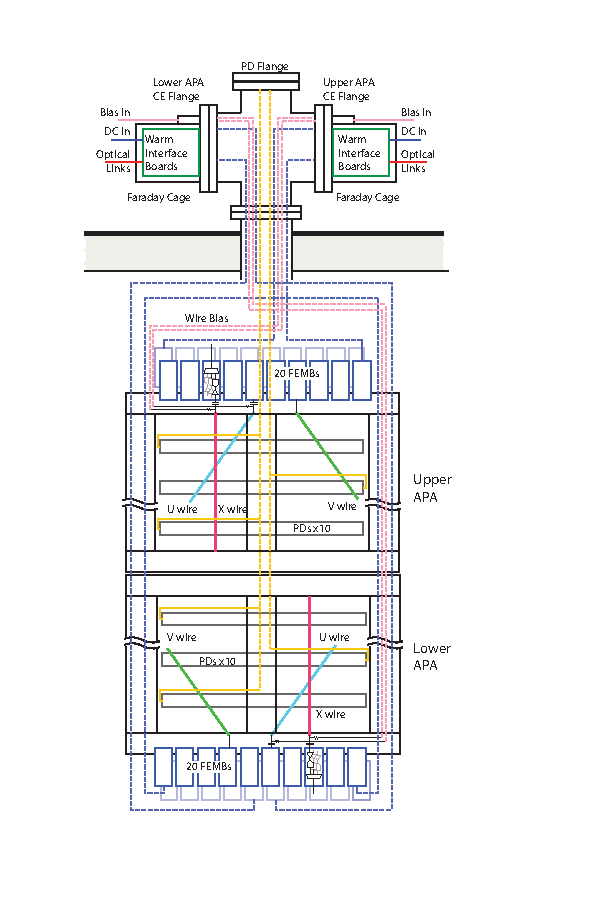
\includegraphics[width=0.7\textwidth]{sp-tpcelec-DUNE-FD-APA-readout-scheme-v1.pdf}
\end{dunefigure}

The components of the \dword{ce} system are the following:
\begin{itemize}
\item{\dwords{femb}, on which the \dwords{asic} are mounted, and 
which are installed on the \dword{apa}s;}
\item{cables for the data, clock, and control signals; \dword{lv} 
power; and wire bias voltages between the \dword{apa} and the 
signal flanges (cold cables);}
\item{signal flanges with a \dword{ce} \fdth to pass the data, clock, 
and control signals; \dword{lv} power; and \dword{apa} wire-bias 
voltages between the inside and outside of the cryostat; and 
the corresponding cryostat penetrations and spool pieces;}
\item{\dwords{wiec} mounted on the signal flanges and contain
the \dwords{wib} and \dword{ptc}s for further processing
and distribution of the signals entering and exiting the cryostat;}
\item{cables for \dword{lv} power and wire bias voltages between 
the signal flange and external power supplies (warm cables); and}
\item{\dword{lv} power supplies for the \dword{ce} and bias-voltage 
power supplies for the \dword{apa}s.}
\end{itemize}

\begin{dunetable}
[TPC electronics components and quantities for a single \dword{apa} of a \dword{spmod}.]
{llr}
{tab:elecNums}
{TPC electronics components and quantities for a single \dword{apa} of the DUNE \dword{spmod}.}
\textbf{Element} &\textbf{Quantity} & \textbf{Channels per element}\\ \toprowrule
Front-end mother board (\dword{femb}) & \num{20} per \dword{apa} & \num{128} \\ \colhline
FE \dword{asic} chip & \num{8} per \dword{femb} & \num{16} \\ \colhline
\dword{adc} \dword{asic} chip & \num{8} per \dword{femb} & \num{16} \\ \colhline
\dword{coldata} \dword{asic} chip & \num{2} per \dword{femb} & \num{64} \\ \colhline
Cold cable bundle & \num{1} per \dword{femb} & \num{128} \\ \colhline
Signal flange & \num{1} per \dword{apa} & \num{2560} \\ \colhline
\dword{ce} \fdth & \num{1} per \dword{apa} pair & \num{2560} \\ \colhline
Warm interface board (\dword{wib}) & \num{5} per \dword{apa} & \num{512} \\ \colhline
Warm interface electronics crate (\dword{wiec}) & \num{1} per \dword{apa} & \num{2560} \\ \colhline
Power and timing card (\dword{ptc}) & \num{1} per \dword{apa} & \num{2560} \\ \colhline
\end{dunetable}

While the higher charge carrier mobility at \dword{lar} temperature than at room
temperature is central to improving the performance of \dword{ce}, it also leads
to the hot carrier effect~\ref{Li:CELAr}. In n-type \dword{cmos} transistors, the carriers (electrons)
can acquire enough kinetic energy to ionize silicon in the active channel. This
charge can become trapped and lead to effects (including threshold shifts)
similar to those caused by radiation damage. This effect can cause \dword{cmos}
circuits to age much more quickly at \dword{lar} temperature than at room temperature,
reducing performance and potentially causing failure. To mitigate this effect,
the maximum \efield in transistor channels must be lower than the field that
can be reliably used at room temperature. This is accomplished by using transistors
fabricated with channel lengths that are larger than the length commonly used
for \dwords{asic} using the same technology, and operated at reduced bias voltage. 
Any commercial circuits used in the \dword{lar} must be carefully tested to ensure 
they will perform well for the expected \dunelifetime lifetime of \dword{dune}; 
reliability studies for front-end electronics designs in consideration are 
discussed in Section~\ref{sec:fdsp-tpcelec-qa-reliability}.

The baseline design for the \dword{spmod} TPC electronics calls for three 
types of custom \dwords{asic} inside  the \dword{lar}:
\begin{itemize}
\item{a \num{16}-channel \dword{fe} \dword{asic} for amplification 
and pulse shaping (referred to as \dword{larasic});}
\item{a \num{16}-channel \num{12}-bit \dword{adc} \dword{asic} 
operating at \SI{{\sim}2}{MHz}; and}
\item{a \num{64}-channel control and communications \dword{asic} 
(referred to as \dword{coldata}).}
\end{itemize}

The development of custom \dword{asic} for the read-out of \dword{lar}
\dword{tpc} has been going on at \dword{bnl} for many years, and prototypes
of \dword{larasic} have been used in previous \dword{lar} \dword{tpc}, 
including \dword{microboone} and \dword{pdsp}. \dword{pdsp} is the first
experiment for which the digitization of the charge and the data serialization
have been performed inside the \lar, using the P1-\dword{adc} \dword{asic} 
developed at \dword{bnl} and a \dword{fpga}, since \dword{coldata} was
still under development. Further development of \dwords{asic} for the
\dword{dune} \dword{spmod} are discussed later in Section~\ref{XXXXXX}.

%%%%%%%%%%%%%%%%%%%%%%%%%%%%%%%%%%%
\subsection{ProtoDUNE-SP Results}
\label{sec:fdsp-tpcelec-overview-pdune}

The Single Phase \dword{protodune}-\dword{sp} detector, described 
in Chapter~\ref{ch:sp-execsum}, is a 700~ton fiducial volume 
\dword{lartpc} with 15,360 sense wires that are read out by 
the \dword{ce} system described in Section~\ref{sec:fdsp-tpcelec-qa-facilities-pdune}. 
The system was deployed in a beam line of the CERN Neutrino Platform 
in 2018 and continues to take cosmic event data into 2019. The goal of 
the \dword{pdsp} \dword{tpc} readout was to validate the concept 
and the design of the integrated \dword{apa}+\dword{ce} readout 
and measure the performance of the \dword{ce} system with components 
as close as possible to the final \dword{dune} \dword{tpc} readout.

Each of the six \dword{protodune}-\dword{sp} \dword{apa}+\dword{ce}
readout units consists of 2,560 sense wires, of which 960 are \SI{6}{m} 
long collection wires and 1,600 are \SI{7.4}{m} long induction wires. 
Five of the six \dword{apa}a were tested in a full scale cold box in 
cold gaseous nitrogen (GN$_2$) with a complete \dword{ce} readout system 
identical to the one on the detector before installation in the cryostat,
while the sixth one was installed without first going through the cold
box testing. Figure~\ref{fig:apa2-cycle} shows the \dword{enc}, which 
is the charge in electrons that would have to arrive at the sense 
wires to generate a signal with the \rms measured by the front end 
electronics, as a function of cold cycle time. At a stable temperature of 
\SI{160}{K} the \dword{enc} for all three wire planes is less than 500~e$^-$.

\begin{dunefigure}
[\dword{pdsp} APA2 noise levels measured in GN$_2$ in the CERN cold box]
{fig:apa2-cycle}
{Left Y-axis: ENC (in electrons) for U, V, and X (red, blue, and green 
curves) sense wire planes as a function of time (hours) for the APA \#2 cold 
cycle in GN$_2$ in the CERN cold box; right Y-axis: temperature 
(orange curve) measured at the level of the front-end electronics.}
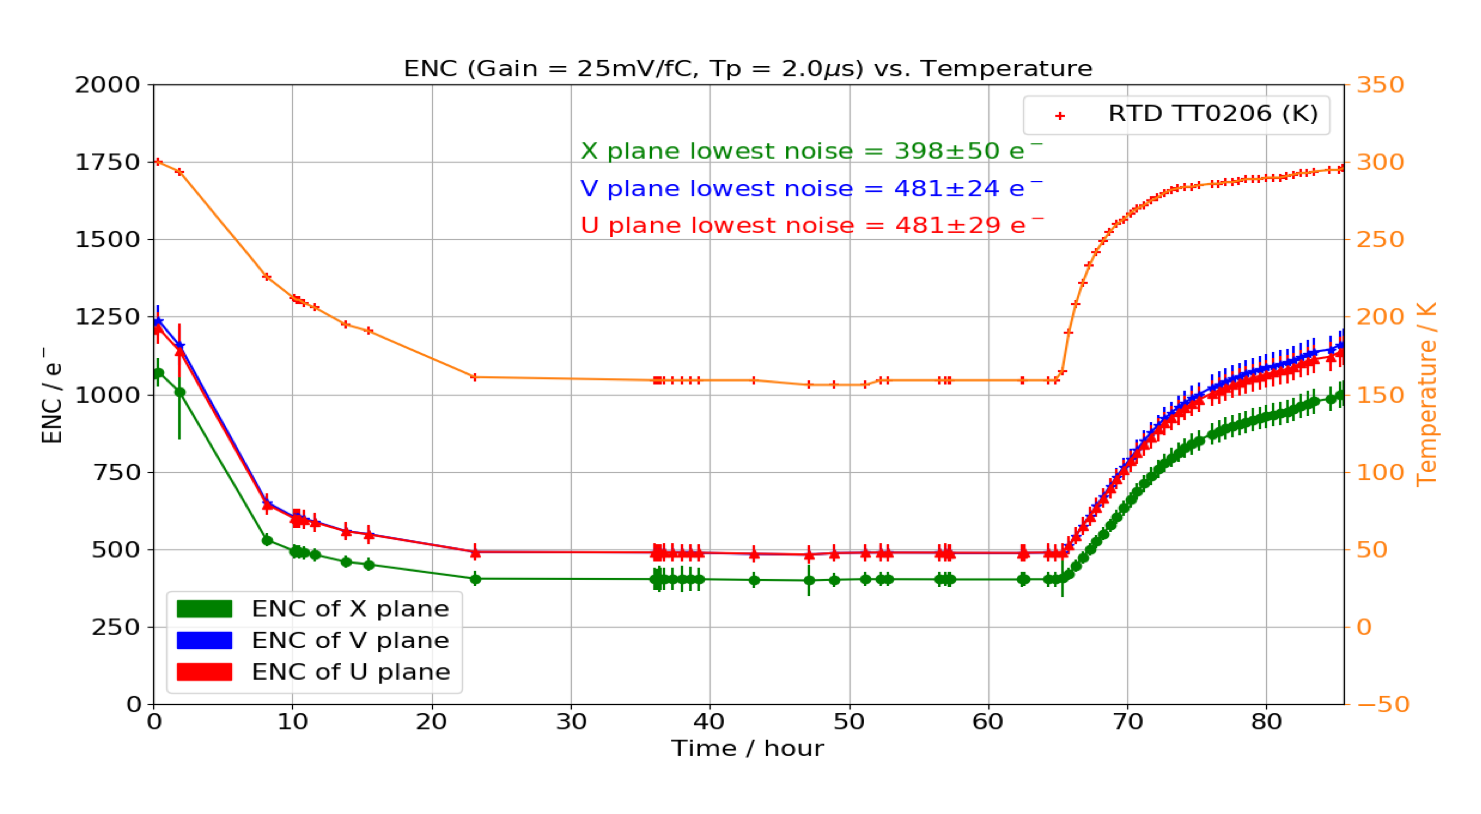
\includegraphics[width=1.0\linewidth]{sp-tpcelec-apa2.png}
\end{dunefigure}

After the cryostat was filled with \dword{lar} and the drift and wire 
bias voltages were set to their nominal values (defined in Chapter~\ref{ch:sp-execsum}), 
99.7\% of the \dword{tpc} readout channels were alive. The following 
channels were expected to be unresponsive to charge deposited on the wires:
\begin{itemize}
\item{Four electronics channels, suggesting a dead channel in the electronics, 
all on collection wires on three different \dwords{apa};}
\item{$\sim$35 channels measured with consistent with no capacitive load 
on the \dword{fe} electronics, suggesting an open connection somewhere in 
front of the \dword{ce} system, scattered randomly throughout the detector 
and on all wire planes.}
\end{itemize}
With the detector in nominal operating conditions, the \dword{enc} 
measured by the online monitoring program was approximately 550~e$^-$ 
on the collection wires and approximately 700~e$^-$ on the induction
wires.averaged over all operational channels. Figure~\ref{fig:apa3-noise} 
shows the \dword{enc} in electrons for all channels of one of the 
\dword{apa}+\dword{ce} readout units. The collection channels with 
\dword{enc}$>$1500~e$^-$ are caused by a problem in the P1-\dword{adc}
\dword{asic} used in \dword{protodune}-\dword{sp}, that had already
been identified at the time of testing the components prior to their
installation on the \dwords{femb}. The channels in all three planes 
with \dword{enc}$<$300~e$^-$ have an open connection somewhere in 
front of the \dword{ce} system.

\begin{dunefigure}
[TPC noise levels measured at \dword{pdsp} after \dword{lar} fill]
{fig:apa3-noise}
{ENC (in electrons) for all U, V, and X (red, blue, and green curves) sense 
wire planes for one ProtoDUNE APA with the detector in nominal operating 
conditions.}
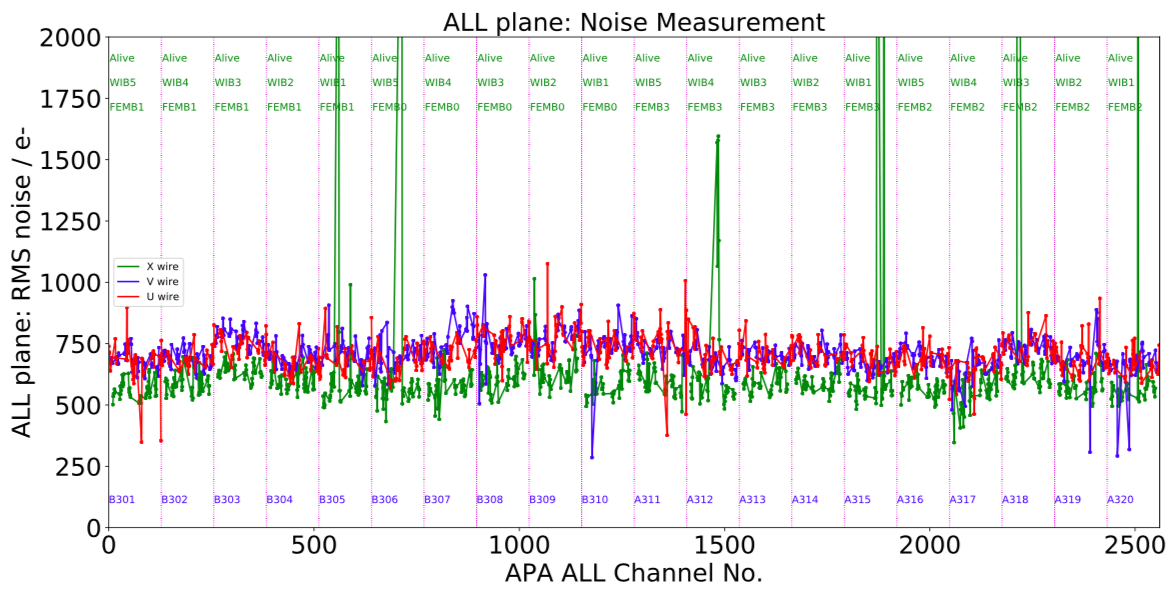
\includegraphics[width=1.0\linewidth]{sp-tpcelec-apa3-enc.png}
\end{dunefigure}

The overall performance of the \dword{ce} system in 
\dword{protodune}-\dword{sp} satisfies the \dword{dune} 
single phase \dword{fd} \dword{ce} system requirements 
listed in Section~\ref{sec:fdsp-tpcelec-overview-requirements}. 
Another demonstration of the performance achieved
and of the progress made since previous detectors based on the
\dword{lartpc} technology is given by a comparison of the raw data from 
a \dword{pdsp} event shown in Figure~\ref{fig:pdsp-display} with
the raw data from a \dword{microboone} event shown in
Figure~\ref{fig:microboone-display}, taken from~\cite{Acciarri:2017sde}.
The \dword{pdsp} event, collected very early in the data taking
period when the charge collection efficiency was still limited
by the amount of impurities in the \dword{lar}, shows very little
noise and appears to be of the same quality as the \dword{microboone}
event display after offline noise removal. This clearly shows
that significant progress has been made in the overall system
design based on the lessons learned from previous experiments
using the \dword{lartpc} technology, resulting in high quality
data with very little noise immediately after the beginning of
data taking.

\begin{dunefigure}
[Raw data from a \dword{pdsp} event]
{fig:pdsp-display}
{Display of the charge deposited on the collection wires (X-axis) as
a function of the drift time (Y-axis) for a \dword{pdsp} event 
that includes two electromagnetic showers and a four-prong interaction.
The color associated with each time sample on the \dword{apa}
wires gives a measurement of the charge measured by the \dword{ce}
readout, increasing from the smallest values (blue) to the largest
ones (red).}
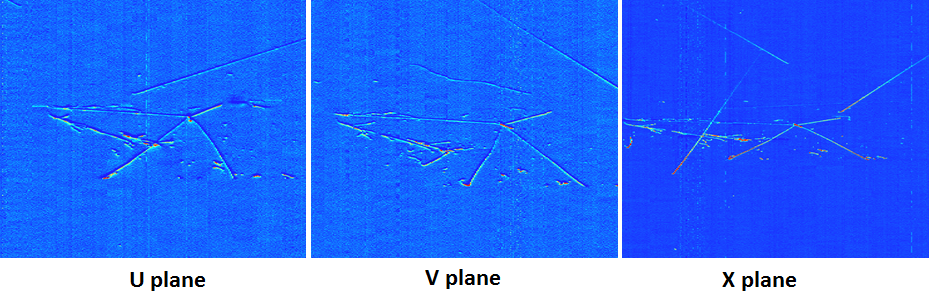
\includegraphics[width=1.0\linewidth]{sp-tpcelec-4prongdisplay.png}
\end{dunefigure}

\begin{dunefigure}
[Raw data from a \dword{microboone} event]
{fig:microboone-display}
{\dword{microboone} 2-D event display of the V plane from run 3493 
event 41075 showing the raw signal (a) before and (b) after offline 
noise filtering. A clean event signature is recovered once all the 
identified noise sources are subtracted. Taken from~\cite{Acciarri:2017sde}.}
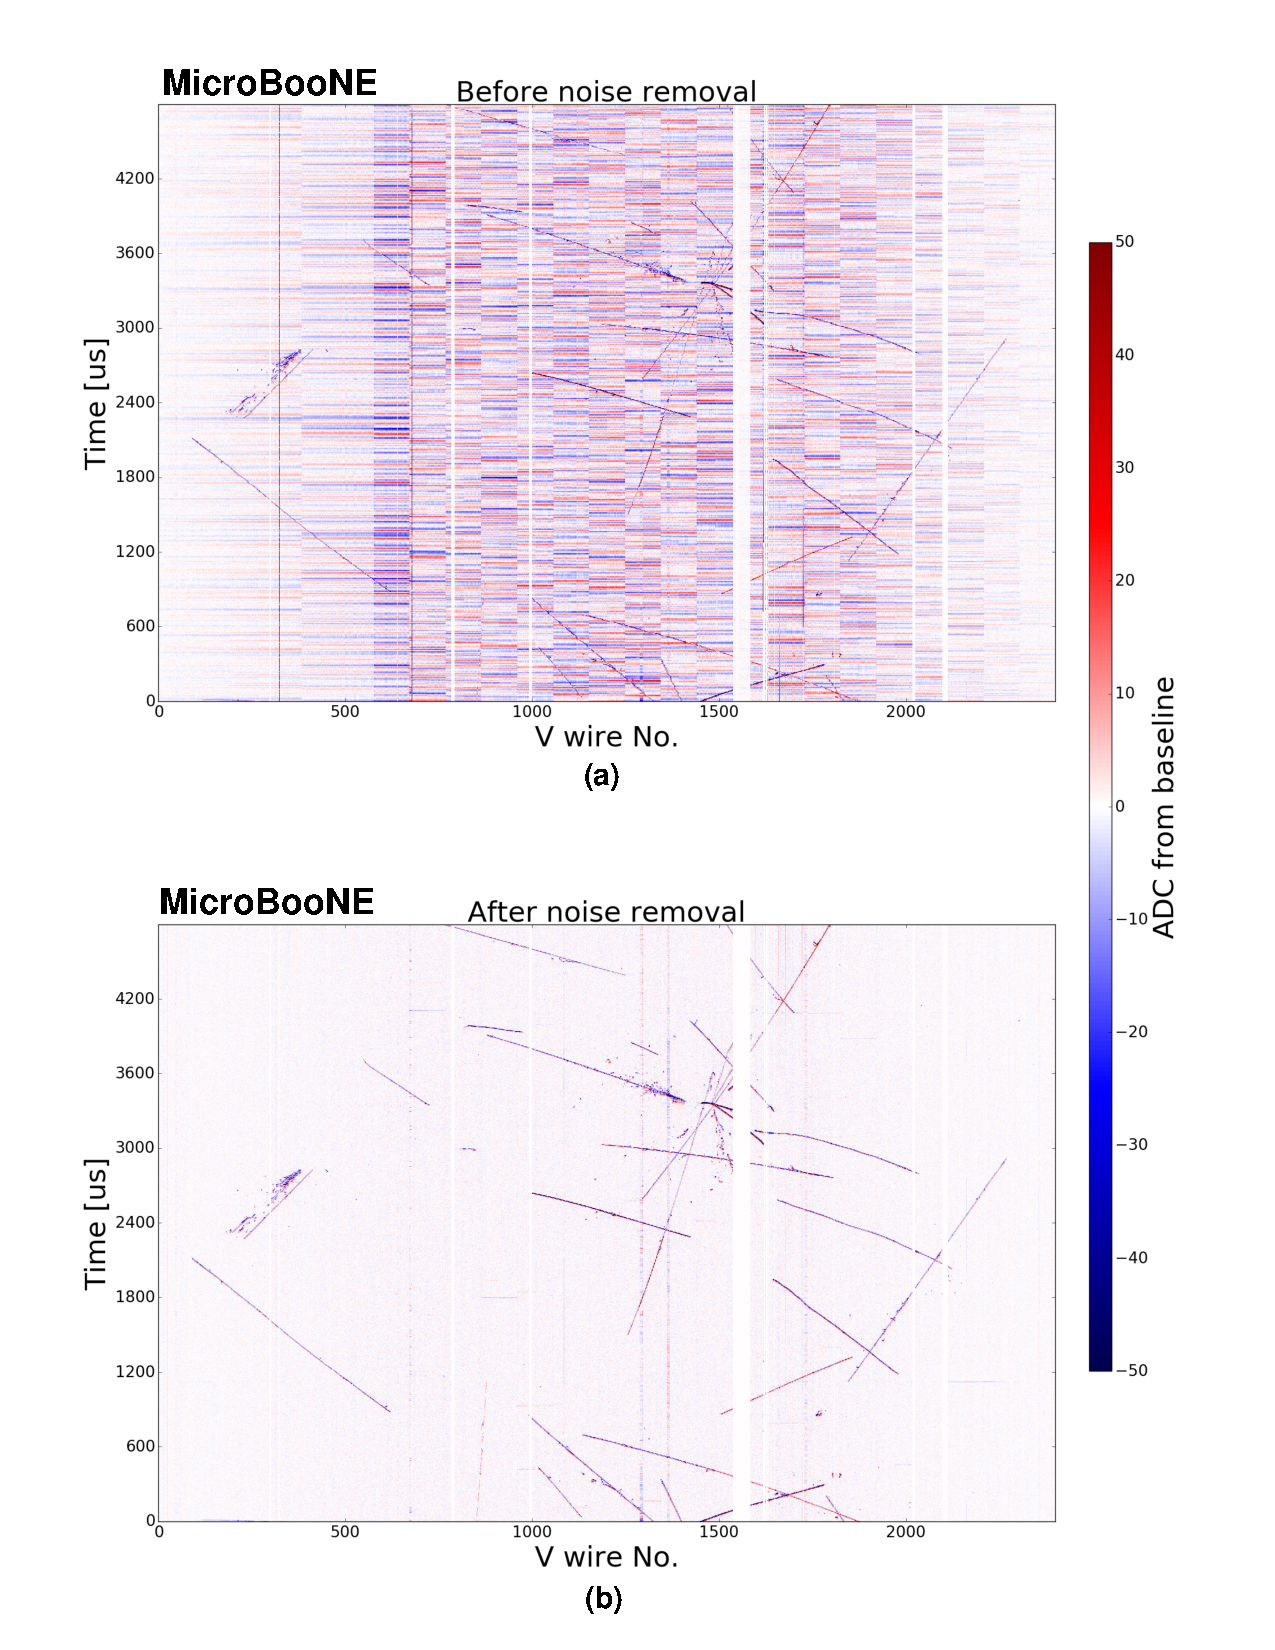
\includegraphics[width=0.9\linewidth]{microBoone_display.pdf}
\end{dunefigure}

%%%%%%%%%%%%%%%%%%%%%%%%%%%%%%%%%%%
\subsection{ProtoDUNE-SP Lessons Learned}
\label{sec:fdsp-tpcelec-overview-lessons}

As discussed in the previous Section, the initial data from \dword{pdsp}
show that the \dword{dune} detector specifications presented in 
Section~\ref{sec:fdsp-tpcelec-overview-requirements} can be met.
However, several improvements and updates to the \dword{ce} system design 
are motivated by the results of the testing and commissioning of, and 
the data-taking with, the \dword{pdsp} electronics. A complete list
of the lessons learned from the construction, testing, integration,
installation, commissioning of the \dword{ce} detector components
is available in~\cite{bib:docdb12367}. In addition to reporting the
lessons learned, the plans and timeline for addressing the issues 
observed in \dword{pdsp} are also discussed in this document. Here
only the main issues are discussed, and the plans for their resolution
are discussed in the next Section, where the planned design changes
for the \dword{dune} detector are discussed.

The main problem with the \dword{pdsp} \dword{ce} readout is in the
P1-\dword{adc} \dword{asic}. This problem was observed already in 2017
when these \dwords{asic} were being tested prior to their installation
on the \dwords{femb}. The main issue with the P1-\dword{adc} is 
that the ``domino'' architecture used in this design relies on
excellent transistor matching, and unfortunately transistor matches
is worse at \dword{lar} temperature. In \dword{pdsp} this problem
results in some readout channels having a fixed value for some of
the \dword{adc} bits. Some these channels need to be masked 
from analysis, resulting in a loss of efficiency for \dword{pdsp}, while
in a majority of cases an approximated value for the charge can
be obtained via interpolation. Due to this problem, plans have
been put in place to develop an \dword{adc} with a completely new
design for \dword{dune}. A new \dword{adc} \dword{asic} (also called 
\dword{coldadc} \dword{asic}) is being developed by an 
\dword{bnl}-\dword{fermilab}-\dword{lbnl} collaboration and first
prototypes are being characterized in February 2019. The design
of this \dword{adc} is discussed in detail in 
Section~\ref{sec:fdsp-tpcelec-design-femb-adc}. In parallel two
alternatives are being considered for \dword{dune}. The first is the
use of \dword{cots} \dword{adc} that has been pursued by the 
\dword{sbnd} collaboration, that is discussed in 
Section~\ref{sec:fdsp-tpcelec-design-femb-alt-cots}. The second is
a single \num{64}-channel \dword{asic} that consolidates
the \dword{fe}, the analog-to-digital conversion, and the
data serialization functionalities in a single chip. This 
development has also reached the prototype stage with \dwords{asic}
being characterized in February 2019. More details about this
solution are discussed in Section~\ref{sec:fdsp-tpcelec-design-femb-alt-cryo}.
At the current time (February 2019) there is already one working
solution that could be adopted for \dword{dune}, the \dword{cots}
solution. Hopefully by Summer 2019 there will also be a demonstration
that one or both of the two custom \dword{asic} solutions satisfy
the \dword{dune} requirements.

Initial analysis of the \dword{pdsp} data has shown a new problem 
with \dword{larasic} The problem occurs when a large amount of 
change ($>$\SI{50}{fC}) is collected over a period of \SIrange{10}{50}{$\mu$s}.
This causes the feedback mechanism of the \dword{fe} amplifier 
to stop working for a certain period of time (several hundred ns). 
In this period, the readout is not functioning and signals following 
the large charge deposited may be completely lost. A ledge is observed 
in the output of the \dword{fe} amplifier, followed by a slow decay 
and a sudden turn-on of the amplifier. An example of this behavior 
from data is shown in Figures~\ref{fig:pdsp-ledge}.

\begin{dunefigure}
[Pulse shape on a \dword{pdsp} wire showing the ledge effect]
{fig:pdsp-ledge}
{Waveform of an event showing the ledge following a large charge 
deposition, then a discharge and a final jump to the normal baseline.}
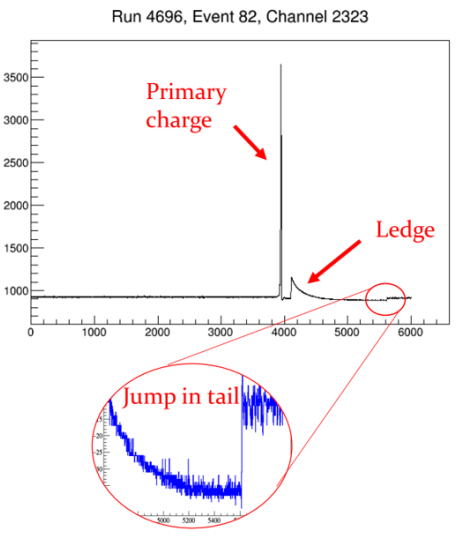
\includegraphics[width=1.0\linewidth]{sp-tpcelec-ledge.png}
\end{dunefigure}

This problem has been reproduced in the laboratory and is being actively 
studied. It affects all versions of \dword{larasic} fabricated after 
the one used for the \dword{microboone} experiment. The problem occurs 
with larger probability for the \SI{200}{mV} baseline used for the collection
wires than for the \SI{900}{mV} baseline used for the induction wires.
After the problem and this difference between the two baselines were 
observed, the decision was taken to operate the \dword{ce} in \dword{pdsp} 
using the \SI{900}{mV} baseline also for the collection wires, sacrificing
the dynamic range. Data from the wires where the problem occurs can
be masked in analysis, resulting in a loss of efficiency. It should be
noted that the problem occurs more often in \dword{pdsp} compared to
\dword{dune} due to the presence of cosmic rays traveling parallel
to the \dword{apa} wires in the first case. The problem cannot be 
discounted for \dword{dune}, since it could also affect the detection
of electromagnetic showers that are one of the main physics signals.
The plan and the timeline for addressing this issue in a new prototype
of \dword{larasic} are going to be discussed in 
Section~\ref{sec:fdsp-tpcelec-design-femb-fe}.

\fixme{need a figure here, will be added on January 29}

\begin{dunefigure}
[Image of a connector for the cold cables lifted from the \dword{femb}]
{fig:pdsp-ledge}
{Image of a connector for the cold readout and signal cables lifted from
the \dword{femb} due to the presence of excess epoxy on the 
connection between the cold cables and the printed circuit board
that acts as the ``male'' part of the connector.}
%% 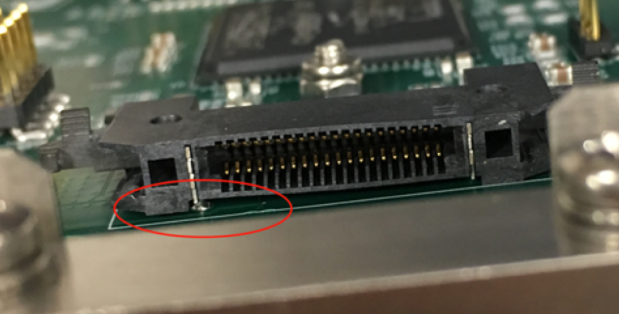
\includegraphics[width=1.0\linewidth]{tpcelec_femb_problem.png}
\end{dunefigure}

During the integration of the \dwords{femb} onto the \dwords{apa}
and the cold tests that preceded the \dwords{apa} installation
inside the \dword{pdsp} cryostat a problem was observed on the 
connection between the cold readout and control cables and the
\dwords{femb}. In multiple cases the connector is detached from
the \dword{femb} causing a loss of communication. This problem 
was fixed for all the \dwords{apa} tested in the cold box by
replacing the \dword{femb}. One additional \dword{femb} was 
replaced on the \dword{apa} that was installed without undergoing 
the test in the cold box. This problem may also be the cause
of the loss of the external clock signal on one of the \dwords{femb}
which was observed after the cool-down of the detector.
The problem has been traced to a mechanical interference between 
the epoxy deposited as a protective measure on the small printed circuit
board to which the cold cables are soldered and which forms the
``male'' part of the connector. The height of the epoxy can cause
the ``female'' part of the connector to lift from, as shown in
Figure~\ref{fig:fdsp-femb-connector}. This problem is being 
addressed by a redesign of the connection between the \dword{femb}
and the cold cables, as discussed in Section~\ref{sec:fdsp-tpcelec-design-femb-overview}.

It should be noted that the analysis of the \dword{pdsp} data
is just starting and that there is a lot to learn about the
detector and how different components of the detector interact
among themselves from data. The level of noise mentioned in
the previous section (approximately \SI{550}{e$^-$} on the collection wires,
and approximately \SI{700}{e$^-$} on the induction wires) 
was obtained from the online data monitoring, without any
filtering or selection applied to the pulses on the \dword{apa}
wires.A simple common mode filter can reduce significantly the 
noise, particularly at low frequencies, as shown in Figure~\ref{fig:pdsp-noise},
that contains the noise spectrum on the three planes of \dword{apa}
wires before and after the filtering. The spectrum prior to
the filtering shows some interesting features. At very low
frequencies $<$\SI{60}{KHz}, the noise is dominated by the
low voltage regulators that are installed on the \dwords{femb}.
The noise from the low voltage regulators has actually
been significantly reduced in \dword{pdsp} compared to
\dword{microboone}~\cite{Acciarri:2017sde}, thanks to 
hardware filters that have been added on the \dword{pdsp} 
\dwords{femb}. The noise spectrum prior to the filtering
also shows spikes at multiple discrete frequencies and in
some cases the noise spectrum have been identified (cameras,
malfunctioning bias voltage supplies). Further data analysis
and further tests with \dword{pdsp} could result in further
improvements of the already excellent \dword{ce} performance
and will be reflected, if appropriate, in changes of the
detector design.

\begin{dunefigure}
[Spectrum of the noise on the \dword{pdsp} \dword{apa} wires before and after noise filtering]
{fig:pdsp-noise}
{Spectrum of the noise on the different \dword{pdsp} \dword{apa} wire planes before
(left) and after (right) applying a simple common mode filter}
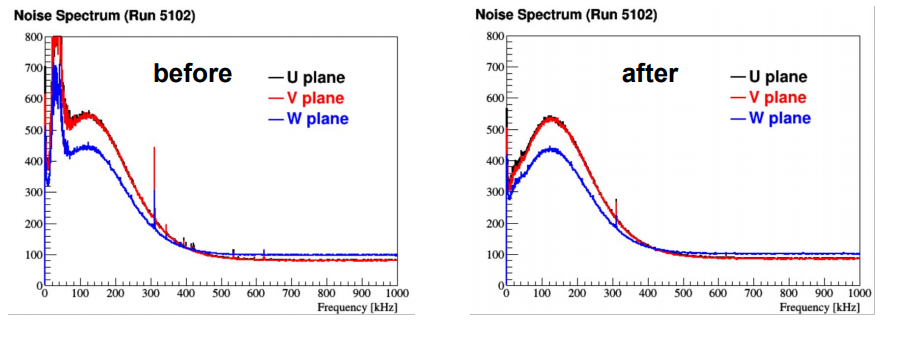
\includegraphics[width=1.0\linewidth]{tpcelec_pdsp_noisespectrum.png}
\end{dunefigure}
